
\chapter{对关联与超流核\label{chap:=005BF9=005173=008054=004E0E=008D85=006D41=006838}}

\section{简介和实验基础}

在第五章我们研究了描述核的基态的波函数。认为基态是直积波函数
\begin{comment}
Slater行列式。
\end{comment}
并且使能量最低，我们就得到了Hartree-Fock方法。正如我们所见，相关方程的解把一组单粒子基转换成了一组更好的单粒子基。变分原理等价于是说要求在基态和最低的激发态-单粒子空穴态之间的矩阵元为零。因此，正如我们在第四章所讨论的，Hartree-Fock方法部分地把相互作用的单粒子-空穴部分也就是说力的长程部分考虑了进去。在我们转而讨论关联导致的激发时，我们需要考虑导致了粒子粒子关联的力的短程部分（见第四章）。我们将会证明，可以通过形式上和单粒子空穴部分的力非常像的方法做到这一点，只需引入“准粒子”构成的广义的直积波函数。

当然我们通常必须同时考虑长程和短程关联，这是在下章的Hartree-Fock-Bogoliubov理论的框架下完成。我们姑且仅仅考虑纯粹的短程（粒子粒子或者对）关联，仅仅如此就能让我们理解Hartree-Fock图像最难以描述的效应。

现在我们总结一下与对关联相关的最重要的实验现象：
\begin{itemize}
\item 能隙。奇核和偶核在形变核的谱上有非常明显的区别。偶偶核只有少数可达$1.5\,\text{MeV}$的（集体）能级。它们可以被很好地描述为转动和振动能带。然而奇偶核非常不一样，它们在相同的能区有许多集体和单粒子态。\ref{fig:=00540C=004F4D=007D20=007684=0080FD=008C31}展示了一些锡同位素的能谱作为例子。
\end{itemize}
\begin{figure}[H]
\begin{centering}
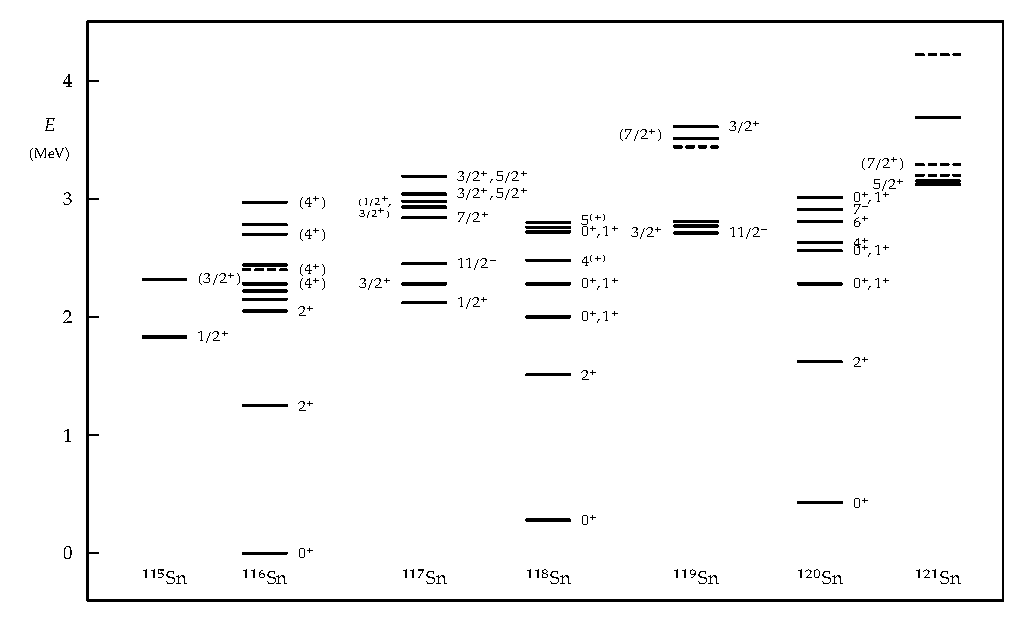
\includegraphics[width=0.65\linewidth]{pictures/6_1}
\par\end{centering}
\centering{}\caption{\label{fig:=00540C=004F4D=007D20=007684=0080FD=008C31}$\ce{_{50}Sn}$同位素的能谱}
\end{figure}

\begin{itemize}
\item 能级密度。如果我们假设在给定$j$下的壳中只有少量核子，由于角动量耦合有各种可能，而耦合得到的态能量都一样，因此是强简并的。单位能量态的数目可以很容易的估计，然而我们发现，在低激发能区域，我们估计的能级密度是实验值的接近两倍。
\item 奇偶效应。一个奇偶核的总结合能比相邻（算术意义上）的两个偶偶核的小。因此我们可以有关于临近核的质量的如下关系：
\[
M_{(A\text{ odd})}>\frac{M_{A-1}+M_{A+1}}{2}
\]

这被称为奇偶效应。
\item 形变原子核的惯性矩可以从旋转带的能级结构中测得。基于单粒子模型推导的结果和实验值差了一个两倍的因子。如果对效应被考虑近来，理论和实验可以很好的符合。
\item 形变。在壳模型里，如果我们对不同的核质量数计算核子密度分布，我们会发现，球对称形状的闭壳核逐渐变成了有大形变的半满壳核。核子数和闭壳核差距不大的核至少在基态的时候都是球形的。逐渐往壳层里填核子，会有一个区域，原子核有非常剧烈的形变，并且在半满的时候达到极大。
\item 低能$2^{+}$态。我们发现在偶数核
\begin{comment}
怀疑是偶偶核。
\end{comment}
里，在闭壳核附近，总是有一个角动量为$2$、宇称为正的能级。这些能级既不可以被解释为旋转能级，也不能被解释为单粒子激发能级。事实上，它们是振动的特征，这和对关联有很强的关系
\end{itemize}
为了理解所有这些现象，我们必须考虑核力短程部分引起的关联。正如在第二章提到的，偶偶核拥有自旋为零的基态，并且奇偶核的自旋可以由奇数核子的角动量确定。这些观察启示Go\"ppert
Mayer\cite{Ma50}做了一些初步的计算，计算显示，对于短程吸引的两体力来说，在一个给定$j$的壳层中，两个核子能量角度上讲更倾向于形成$I=0$的对而不是别的组合。如果忽略自旋，并且考虑$|lm\rangle$态和$|l,-m\rangle$的密度分布，这就可以很容易的理解，正如在\ref{fig:=007ED9=005B9A=0078C1=0091CF=005B50=006570=004E0B=007684=006838=005B50=005BC6=005EA6=005206=005E03}（或者是4.4.7中的讨论）中系统展示的那样。对于这些密度分布，很明显是在两个核子有着相同$|m|$的时候，它们密度的空间分布交叠达到最大。对于一个短程力来说，两个核子$\left|m\right|$相同但符号相反的时候能量是最低的
\begin{comment}
这似乎不是很容易精确证明？
\end{comment}
（它们方向相同的时候明显不符合Pauli不相容原理，在第三章中角动量
\begin{comment}
不知道是啥
\end{comment}
）。这里，符号相反意味着耦合后$I=0$。不考虑前面的系数，核子对的耦合成$I=0$，$M=0$角向部分为：

\begin{figure}[H]
\begin{centering}
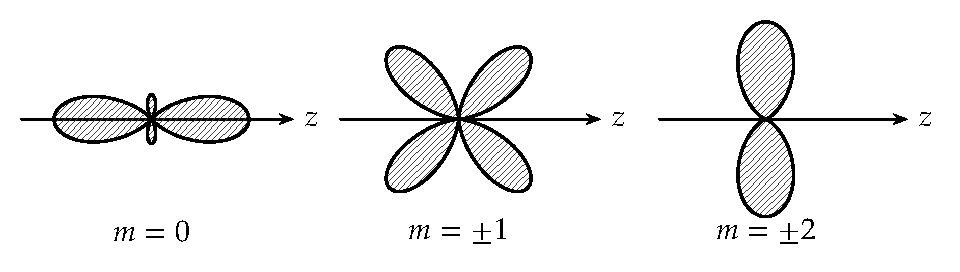
\includegraphics[width=0.6\linewidth]{pictures/6_2}
\par\end{centering}
\centering{}\caption{\label{fig:=007ED9=005B9A=0078C1=0091CF=005B50=006570=004E0B=007684=006838=005B50=005BC6=005EA6=005206=005E03}给定磁量子数下的核子密度分布}
\end{figure}

\begin{align}
\langle\theta_{1}\varphi_{1},\theta_{2}\varphi_{2}|nljjI=0,M=0\rangle & \propto\sum^{l}_{m=-l}(-1)^{m}Y_{lm}(\theta_{1},\varphi_{1})Y_{l,-m}(\theta_{2},\varphi_{2})\label{eq:angular part of pair}\\
 & =\frac{2l+1}{4\mathrm{\pi}}P_{l}(\cos\theta_{12})\nonumber 
\end{align}

这里$\theta_{12}$是两个核子的夹角。
\begin{comment}
这里有点没搞清楚是怎么来的。
\end{comment}
从上式可以看出，核子对的波函数只依赖于相对角度$\theta_{12}$。因此对于一个固定的$\theta_{12}$，核子对的波函数是一个核周围的均匀分布。由于两个核子的径向函数是相同的，通常不能得知关于核子对在空间中的位置更详细的信息，径向依赖性很大程度上是核子波函数的节点结构问题
\begin{comment}
这一句话是什么意思？
\end{comment}
。正如我们在\ref{fig:=009636Legendre=00591A=009879=005F0F=005173=004E8E=005939=0089D2=007684=0051FD=006570}中所看到的，$P_{l}(\cos\theta_{12})$在$\theta_{12}$处有一个宽度为$1/l$的峰。因此，两个核子有在角度上靠近的趋势。由于核力的短程性，这对于空间分布交叠取最大值是必须的。另一方面，因为不确定性原理的限制，两个核子也不能靠的太近。\footnote{可以非常简单的确定，如果$\psi(\boldsymbol{r}_{1},\boldsymbol{r}_{2})\sim\delta(\boldsymbol{r}_{1}-\boldsymbol{r}_{2})$，那么动量将会趋向于无穷大。}我们因此可以说，由于相互作用的短程性，两个核子想靠的尽可能的近，然而动能又想使核子分开，两者之间有一个妥协。

如果$j$壳层有不止一对核子， 泡利原理会稍微阻碍（$I=0$）电子对的形成，因为一些成对所需的$m$态已经被另一对核子占据。这种对的相互作用产生了某些特殊的性质，我们将在后面研究，但这并不破坏$j$壳层的处于的成对态的性质。此外，一些跃迁概率这样的典型性质与我们在给定的$j$壳层中拥有的对的数目成正比。如果我们考虑粒子和空穴之间的对称性，即既考虑粒子-粒子对也考虑空穴-空穴对，那么半满壳层是集体性最大的情况
\begin{comment}
这里集体性最大是什么意思？
\end{comment}
，而闭壳核则不可能形成对。
\begin{comment}
为什么？
\end{comment}

对于闭壳核之外的核，能量最低的态应当是所有核子都成对的态（除了奇偶核情况下的最后一个核子
\begin{comment}
奇奇核呢？
\end{comment}
）。为了激发偶偶核，我们必须打破一个对，然而对于奇偶核则只需要把单独的那个核子放到一个很低的能级上。由于对的结合能是$1-2\,\text{MeV}$，因此偶偶核和奇偶核第一激发态和基态的能量差就可以被定性的解释了。

其它上面提到的现象也可以利用对模型理解。由于偶偶核能谱底部能隙的存在，能级密度和实验符合的好多了，奇偶效应由此也非常显而易见。正如我们\ref{eq:angular part of pair}中看到的，$I=0$的对更倾向于球形（即没有方位偏好）。因此，由于对效应阻碍了形变，闭壳核附近的核也是球形的。而在远离闭壳核时则不是球形。事实上，更为精确的描述非常依赖于对力相对于长程（p-h）力的强度。尽管如此，从球形核到形变核的这一突变已经是可以理解的了。

与之紧密相关的还有开壳偶偶核能谱底部$2^{+}$态的存在。因为回复力，也即对效应和形变效应的差，非常小，闭壳核附近的球形核可以很容易激发出一个在它们平衡位形附近的形状振动。因此这些核会形变成一个椭球并且在球形附近以一个很低的频率振动（振动能级$2^{+}$）。

对相互作用的对角化并不能解释为像Hartree-Fock势那样的形式的平均静态能量的贡献。它是一种全新的效应，导致了所谓的对势。这一现象和金属中的超导现象类似。这就是Bohr，Mottelson和Pines\cite{BMP58}和Belyaev\cite{Be59}成功把Barden,
Cooper和Schrieffer{[}BCS 57{]}关于超导的理论应用于原子核的原因。

\section{辛弱数模型\label{sec:6.2_Seniority=0065B9=006848}}

正如我们在引言中说的，对关联是由于核子核子相互作用中的短程部分，并且这个相互作用对$I=0$的对最有效。在4.4.7节我们研究了一下这个问题；为了更进一步的研究对现象，我们考虑\ref{eq:pure pairing force}中的模型力，并考虑$N$个处在$2j+1$重简并的$j$壳的粒子，通过这个模型力相互作用。如果我们令$j$壳的能量为零，相应的
Hamilton 量应该具有这种形式\footnote{注意到接下来我们使用了BCS相位\ref{eq:BCS phases}。}：
\begin{equation}
H=-G\sum_{m,m^{\prime}>0}a^{\dagger}_{m^{\prime}}a^{\dagger}_{-m^{\prime}}a_{-m}a_{m}=-GS_{+}S_{-}\label{eq:Seniority Hamiltonian}
\end{equation}

这里：
\begin{equation}
S_{+}=\sum_{m>0}a^{\dagger}_{m}a^{\dagger}_{-m};\quad S_{-}=(S_{+})^{\dagger}\label{eq:quasi spin ladder operator}
\end{equation}

我们引入这两个算符，是因为它们可以被认为是假想的角动量的升降算符，我们称之为准自旋（就如同第五章中Lipkin模型中的情况）。它和真正的自旋没有任何关系，但是引入它对\ref{eq:Seniority Hamiltonian}的求解很有帮助\cite{Ke61}。同样是为了方便求解，我们继续对每个态$m(m>0)$都引入三个量：
\begin{align*}
s^{(m)}_{+} & =a^{\dagger}_{m}a^{\dagger}_{-m}\\
s^{(m)}_{-} & =a_{-m}a_{m}\\
s^{(m)}_{0} & =\frac{1}{2}(a^{\dagger}_{m}a_{m}+a^{\dagger}_{-m}a_{-m}-1)
\end{align*}

理由算符$a_{m}$和$a^{\dagger}_{m}$的对易关系，我们可以推导出相应的对易关系：
\begin{align*}
[s^{(m)}_{+},s^{(m)}_{-}] & =2s^{(m)}_{0}\\{}
[s^{(m)}_{0},s^{(m)}_{+}] & =s^{(m)}_{+}\\{}
[s^{(m)}_{0},s^{(m)}_{-}] & =-s^{(m)}_{-}
\end{align*}

因此我们发现$s^{(m)}_{+},s^{(m)}_{-},s^{(m)}_{0}$有着和角动量算符相同的对易关系。$s^{(m)}_{+}$和$s^{(m)}_{-}$是和$j_{+}$与$j_{-}$类比的升降算符。而$s^{(m)}_{0}$是和$j_{0}$类比的$z$方向的角动量算符。我们因此可以看出我们为什么称$\boldsymbol{s}^{(m)}$为$m$能级的准自旋算符了。

从$s^{(m)}_{0}$的定义中我们还可以发现它的本征值是$\pm\frac{1}{2}$，和$(m,-m)$是否是占据的有关。因此$\boldsymbol{s}^{(m)}$在$m$能级
\begin{comment}
原书为$j$-level。
\end{comment}
有零个或两个粒子的时候准自旋为$\frac{1}{2}$。如果只有一个粒子，那么$\boldsymbol{s}^{(m)}$的所有分量都为零，因此$\boldsymbol{s}^{(m)}$准自旋为零。

总准自旋算符$\boldsymbol{S}$定义为：
\begin{equation}
\boldsymbol{S}=\sum_{m>0}\boldsymbol{s}^{(m)}\label{eq:total quasi spin operator}
\end{equation}

这当然也是一个角动量算符，由此对 Hamilton 量\ref{eq:Seniority Hamiltonian}可以方便地写为：
\[
H=-G(\boldsymbol{S}\cdot\boldsymbol{S}-S^{2}_{0}+S_{0})
\]

我们又注意到：
\begin{equation}
S_{0}=\frac{1}{2}\sum_{m>0}(a^{\dagger}_{m}a_{m}+a^{\dagger}_{-m}a_{-m}-1)=\frac{1}{2}(\hat{N}-\Omega)\label{eq:S0}
\end{equation}

这里$\Omega=j+\frac{1}{2}$，是该壳层可能存在的对的数目
\begin{comment}
原书仅为“对的数目”。
\end{comment}
。因此$S_{0}$的本征值是整数或者半整数。进一步，根据角动量代数的性质我们可以得到：
\[
S\geq\left|S_{0}\right|=\frac{1}{2}\left|N-\Omega\right|
\]

根据\ref{eq:total quasi spin operator}，$S$的最大值是$S=\Omega/2$，因此我们可以看出$S$可以取$\Omega/2,\Omega/2-1,\Omega/2-2,\dots,\left|\Omega/2-N/2\right|$中的所有值。于是一个态可以用$S$和$S_{0}$标记，能量本征值因此为：
\[
E(S)=-G[S(S+1)-\frac{1}{4}(N-\Omega)^{2}+\frac{1}{2}(N-\Omega)]
\]

为了替代准自旋$S$，我们也可以引入一个量子数——辛弱数$s$\cite{Ra43}。它由下式给出：
\[
S=\frac{1}{2}(\Omega-s)
\]

这里：
\begin{align*}
s & =0,2,4,\dots,N\quad\text{如果}N\text{是偶数}\\
s & =1,3,5,\dots,N\quad\text{如果}N\text{是奇数}
\end{align*}

总能量关于辛弱数的关系可以如下给出：
\begin{align}
E(N,s) & =-\frac{G}{4}(N-s)(2\Omega-s-N+2)\nonumber \\
 & =-\frac{G}{4}(s^{2}-2s(\Omega+1)+2N(\Omega+1)-N^{2})\label{eq:E to seniority}
\end{align}

这一力的典型特点是能量的表达式中只有辛弱数量子数，而对其它所有量子数（除了$N$）都是简并的。此外，尽管能量的值强烈依赖于粒子数，谱并不如此。由于相邻能级的总准自旋差$1$，因此能量差为：
\begin{equation}
E(S-1)-E(S)=2GS\label{eq:energy difference to S}
\end{equation}

给定$N$，结合能随$S$增大而增加，因此基态就是所有的准自旋同向的情况，也就是说$S=\frac{1}{2}\Omega$或者$s=0$的情况。对于一个偶数粒子数的系统，第一个激发态的$s=2$，从\ref{eq:E to seniority}或\ref{eq:energy difference to S}我们可以得到：
\begin{equation}
E(N,s=2)-E(N,s=0)=G\Omega\label{eq:energy gap}
\end{equation}

因此激发能与$j$壳的粒子数无关。

如果我们在$j$壳只有两个粒子，辛弱数可以取$s=0,2$。两个全同核子可以耦合成$I=0,2,4,\dots,2j-1$。而只有$I=0$的态被影响了——它的能量被对相互作用降低了。其它的态都没有被影响，因此是简并的。因此我们看到基态（$s=0$）有$I=0$而激发态（$s=2$）有$I=2,4,6,\dots$，这意味着在基态，两个核子“成对”了，而在激发态发生了“拆对”。在\ref{fig:(a)=007EAF=005BF9=00529B=007684=004E24=007C92=005B50=008C31=003002(b)210Po=007684=0080FD=008C31}中展示了这一事实，同时为了比较，我们也展示了$\ce{^{210}Po}$（$1h9/2$壳中有两个中子）的低激发谱。一般的，基态结合能关于$N$的函数可以写成：
\begin{equation}
E(N,s=N)-E(N,s=0)=-E(N,s=0)=G\Omega\frac{N}{2}\left(1-\frac{N-2}{2\Omega}\right)\label{eq:E to N}
\end{equation}

\begin{figure}[H]
\begin{centering}
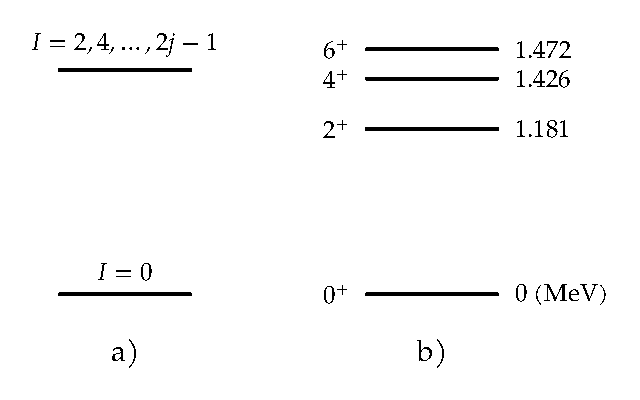
\includegraphics[width=0.65\linewidth]{pictures/6_3}
\par\end{centering}
\centering{}\caption{\label{fig:(a)=007EAF=005BF9=00529B=007684=004E24=007C92=005B50=008C31=003002(b)210Po=007684=0080FD=008C31}(a)纯对力的两粒子谱。(b)$\ce{^{210}Po}$（$1h9/2$壳中的2$p$）的能谱}
\end{figure}

可以看出，当粒子数远小于壳的简并度的时候，结合能随对的数目（$n=N/2$）是线性增长的，也就是说总能量就是一个对的结合能乘上对的数目。如果我们画出基态能量关于$n$的函数，我们将会得到一个谐振子谱\ref{fig:=005BF9=00632F=0052A8=007684=008C10=00632F=005B50=008C31}。这就是对振动谱，在诸如铅附近的区域被发现，我们将会在8.3.5广泛的讨论这一点。所有的\ref{fig:=005BF9=00632F=0052A8=007684=008C10=00632F=005B50=008C31}中的态都是准自旋最大的态（$s=0$），也就是基态，我们称之为$s=0$带。当然，这意味着也有$s=2$带等等。可以得到，两粒子在同一个带的不同态之间跃迁比在不同带间更容易
\begin{comment}
可能在后面有？
\end{comment}
。如果对的数目增加，由于Pauli不相容原理，$I=0$对的互相干扰会变得重要，因此谱\ref{eq:E to N}不再是谐振子的。

\begin{figure}[H]
\begin{centering}
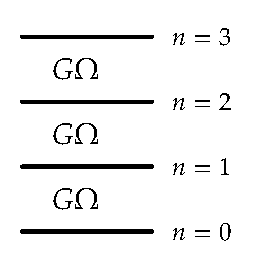
\includegraphics[width=0.4\linewidth]{pictures/6_4}
\par\end{centering}
\centering{}\caption{\label{fig:=005BF9=00632F=0052A8=007684=008C10=00632F=005B50=008C31}对振动的谐振子谱}
\end{figure}

我们可以看出，第一激发态的激发能和一个对的结合能相同，因此我们也可以说在第一激发态（$s=2$）两个核子拆对了。（不可能通过使对激发到能量更高的态上来得到第一激发态，因为我们的模型中只有一个能级。）推而广之，我们可以说辛弱数$s$的态有$s$个未成对的粒子（不论$s$是奇的还是偶的）。

显然，基态一定是非简并的，因为只有一种方式使得$\Omega$个$\frac{1}{2}$准自旋耦合成$S=\Omega/2$总准自旋。而要耦合出$s=2$的态却有$\Omega-1$种方式：
\[
t_{2}=\Omega-1=\begin{pmatrix}\Omega\\
1
\end{pmatrix}-\begin{pmatrix}\Omega\\
0
\end{pmatrix}
\]

考虑一个例子会更方便理解，例如$\Omega=4$。$s=2$的态可以表示为$\overset{1}{\rightarrow}\overset{2}{\rightarrow}\overset{3}{\rightarrow}\overset{a}{\leftarrow}$。有$4-1=3$种可能性把$a$和其它准自旋组合在一起，分别是$a1,a2,a3$。

可以确定，对任意偶数$s$，简并度可以由下式给出\cite{BS68a}：
\[
t_{s}=\begin{pmatrix}\Omega\\
s/2
\end{pmatrix}-\begin{pmatrix}\Omega\\
s/2-1
\end{pmatrix},\quad s\leq N
\]

辛弱数 Hamilton 量\ref{eq:Seniority Hamiltonian}对应的波函数也可以通过准自旋得到。对于$N=0$（空壳）和$N=2\Omega$（满壳），准自旋的第三分量分别全为$-\frac{1}{2}$或$\frac{1}{2}$。因此，真空态是$S=\frac{1}{2}\Omega,S_{0}=-\frac{1}{2}\Omega$的态：
\[
|\rangle=|\frac{1}{2}\Omega,-\frac{1}{2}\Omega\rangle
\]

满壳是$S=\frac{1}{2}\Omega,S_{0}=\frac{1}{2}\Omega$的态$|\Omega/2,\Omega/2\rangle$。如果我们用$|SS_{0}\rangle$表示任意一个准自旋态（这里$S_{0}=\frac{1}{2}(N-\Omega)$），不同偶数$N$的基态（$S=\Omega/2$）可以写为：
\begin{equation}
|\frac{1}{2}\Omega,S_{0}\rangle=|\frac{1}{2}\Omega,\frac{N-\Omega}{2}\rangle\propto S^{N/2}_{+}|\rangle\label{eq:ground state of seniority model}
\end{equation}

$S_{+}$的每次作用使得粒子数提高$2$。基态是$S^{2}$和$S_{0}$和$H$的本征态， 并且仅仅是$n=N/2$个对态的乘积。因此，我们可以说基态是对凝聚。

对于奇粒子系统，最后总有一个粒子无法成对，所以有一个准自旋必须为零。由此$S$可能的最大值将是$\frac{1}{2}(\Omega-1)$，基态为：
\[
|\frac{\Omega-1}{2},S_{0}\rangle\propto S^{\frac{1}{2}(N-1)}_{+}a^{\dagger}_{m}|\rangle
\]

由于$m$可以取$2\Omega$个不同的值$-j\leq m\leq j$，奇$N$粒子系统的基态因此是$2\Omega$简并的（与偶核的非简并相反）。这可以解释为什么奇核的基态附近能级密度很大，而偶核基态总是存在一个能隙。

正如我们已经看到的那样，辛弱数为2的态（$S=\frac{1}{2}\Omega-1$）是偶粒子的第一激发态。它们也可以用准自旋算符构建。

我们首先考虑$N=2$的情况，利用以下算符构建具有好的角动量量子数的态：
\[
A^{\dagger}_{IM}=\frac{1}{\sqrt{2}}\sum_{m_{1}m_{2}}C^{jjI}_{m_{1}m_{1}M}a^{\dagger}_{m_{1}}a^{\dagger}_{m_{2}}
\]

将其作用到真空态即可：
\begin{equation}
|IM\rangle=A^{\dagger}_{IM}|\rangle\label{eq:|IM>}
\end{equation}

由于$A^{\dagger}_{00}\propto S_{+}$（我们利用BCS相，\ref{eq:BCS phases}）,它们是准自旋算符的本征态，对$I=0$，有$S=\Omega/2$，对$I\neq0$，则有$S=\frac{1}{2}\Omega-1$。为了看出这一点，我们计算：
\[
S^{2}|IM\rangle=[S^{2},A^{\dagger}_{IM}]|\rangle+\frac{1}{2}\Omega\left(\frac{1}{2}\Omega+1\right)|IM\rangle
\]

右边第一项为：
\begin{align*}
[S^{2},A^{\dagger}_{IM}]|\rangle & =[S_{+}S_{-},A^{\dagger}_{IM}]|\rangle+[S^{2}_{0}-S_{0},A^{\dagger}_{IM}]|\rangle\\
 & =S_{+}[S_{-},A^{\dagger}_{IM}]|\rangle+[S^{2}_{0}-S_{0},A^{\dagger}_{IM}]|\rangle
\end{align*}

由于$S_{-}$正比于$A_{00}$，可以从Clebsch-Gordon系数的正交关系\cite{Ed57}中得到，对于$I\neq0$：
\[
[S_{-},A^{\dagger}_{IM}]|\rangle=0
\]

利用\ref{eq:S0}，我们最终得到对于$I\neq0$的情况来说：
\begin{align*}
S^{2}|IM\rangle & =-\Omega|IM\rangle+\frac{\Omega}{2}\left(\frac{\Omega}{2}+1\right)|IM\rangle\\
 & =\left(\frac{\Omega}{2}-1\right)\frac{\Omega}{2}|IM\rangle
\end{align*}

因此，两粒子态$|IM\rangle$在$I\neq0$的情况下是$S^{2}$的本征值为$S=\Omega/2-1$（或$s=2$）的本征态，也就是说，这两个粒子在$I\neq0$的情况下是不成对的。

由于算符$S_{+}$不改变$S$，只增加两个粒子，因此很容易构建偶$N$粒子系统（$N>2$）的第一激发态：
\[
|\frac{1}{2}\Omega-1,S_{0}\rangle\propto S^{\frac{1}{2}(N-2)}_{+}A^{\dagger}_{IM}|\rangle
\]

由于$S_{+}$是二阶球张量，因此这些$I\neq0$的态的角动量量子数为$I,M$，辛弱数为$2\text{。}$

当然，这些态是Hamilton 量\ref{eq:Seniority Hamiltonian}的本征能量为\ref{eq:E to seniority}的本征态。我们可以看出能量不依赖于$I,M$。正如我们之前说明的，更高的激发态是由未成对的粒子数标记的，也就是辛弱数$s$。这样的态可以通过算符$A^{\dagger}_{IM}$的相乘很容易的得到，但是样构造的态与低激发态的正交性，以及角动量守恒的特性并不显然。

许多情况下，我们并不需要精确构造波函数（例如，许多矩阵元可以通过角动量耦合的技巧得到。），这也是准自旋这套框架的优点。

举个例子，我们尝试计算四极算符的矩阵元：
\begin{align*}
Q_{20} & =\sum^{n}_{m=-j}q_{m}a^{\dagger}_{m}a_{m}=\sum_{m>0}q_{m}s^{(m)}_{0}\\
q_{m} & =\langle jm|r^{2}Y_{20}|jm\rangle
\end{align*}

由上式我们可以看出$Q_{20}$在准自旋空间是一个矢量
\begin{comment}
什么意思？
\end{comment}
。这一事实意味着四极算符的矩阵元关于对$S_{0}=\frac{1}{2}(N-\Omega)$的依赖（也就是对粒子数的依赖）可以由Wigner-Eckart定理\cite{Ed57}给出：
\[
\langle SS_{0}|Q_{20}|S^{\prime}S_{0}\rangle=(-)^{S-S_{0}}\begin{pmatrix}S & 1 & S^{\prime}\\
-S_{0} & 0 & S_{0}
\end{pmatrix}\langle S||Q_{2}||S^{\prime}\rangle
\]

由于四极跃迁是从辛弱数$s=0$的基态到$s=2$的激发态（由上式的选择定则给出），我们得到四极跃迁概率：
\begin{align*}
\left|\langle s=2|Q_{20}|s=0\rangle\right|^{2} & \propto\begin{pmatrix}\Omega/2 & 1 & \Omega/2-1\\
-S_{0} & 0 & S_{0}
\end{pmatrix}^{2}\propto\left(\frac{\Omega}{2}-S_{0}\right)\left(\frac{\Omega}{2}+S_{0}\right)=\frac{N}{2}\left(\Omega-\frac{N}{2}\right)
\end{align*}

从上式我们可以看出在引言中提到的跃迁概率的集体效应：它正比于核子对数$N/2$和空穴对数$(\Omega-N/2)$的乘积。因此，由于前面提到的基态的对的凝聚，集体效应在闭壳层的中间最为显著。实验上也发现闭壳层中间的核四极跃迁概率显著比壳模型计算的结果要高，我们与之符合的很好。

这一节我们提出的模型实际上非常简单，实际上情况当然要复杂的多。例如，我们必须考虑更多的能级和更现实的核力。尽管如此，我们想强调的是辛弱数模型的许多特点在更实际的情况下也是存在的，此外，这一模型在数学和物理上的简明性也比更为抽象的准粒子框架更好的反映了实际情况。准粒子框架正是我们下一节要介绍的，我们通常用它来处理更为复杂的情形。

\section{BCS模型}

\subsection{波函数}

辛弱数模型不紧急可以用在$j^{N}$组态。如果存在一些闭壳核芯上一些接近简并的$j$-壳，这一模型也可以推广\cite{Ta71,Ta76,LA74,Lo75}。然而，在远离闭壳核的情况下，原子核形变很大，能级也不再是均匀分布，辛弱数模型就完全失效了。

然而，辛弱数模型的结果告诉我们原子核中的对关联在开壳中是十分重要的，有理由相信远离闭壳核的时候这依然是正确的。接下来我们提出一个方法，这一方法既可以处理原子核中所有的核子，也可以简单的推广到不同类型的相互作用的情况。这一方法不能提供一个本征值问题的精确解，但是它像Hartree-Fock一样可以从变分原理得到。因此，对基态波函数做一个正确的拟设是很重要的。类比Bardeen，Cooper和Schrieffer\cite{BCS57}在超导问题中给出的基态，我们试着把偶偶核的基态表示成：
\begin{equation}
|\text{BCS}\rangle=\prod_{k>0}(u_{k}+v_{k}a^{\dagger}_{k}a^{\dagger}_{\bar{k}})|\rangle\label{eq:BCS wave function}
\end{equation}

这里$u_{k}$和$v_{k}$是变分参数。这里的乘积取遍了一半的组态空间，用$k>0$表示。对每一个大于零的$k$态，都有一个共轭态$\bar{k}<0$，并且$\{k,\bar{k}\}$生成了整个单粒子态空间。

$v^{2}_{k}$和$u^{2}_{k}$代表了一个对$(k,\bar{k})$占据或不占据的概率，它们是令能量期望值最小得到的。它们不是独立的，上述态归一化的要求给出：
\begin{equation}
|u_{k}|^{2}+|v_{k}|^{2}=1\label{eq:normalization of BCS}
\end{equation}

\begin{booknote*}
归一化使得：
\begin{align*}
\langle\text{BCS}|\text{BCS}\rangle & =\langle|\prod_{i>0}(u^{*}_{i}+v^{*}_{i}a_{\bar{i}}a_{i})\prod_{i^{\prime}>0}(u_{i^{\prime}}+v_{i^{\prime}}a^{\dagger}_{i^{\prime}}a^{\dagger}_{\bar{j}})|\rangle\\
 & =\prod_{i>0}(|u_{i}|^{2}+|v_{i}|^{2})=1
\end{align*}

因此一个可选的方案就是令$|u_{i}|^{2}+|v_{i}|^{2}=1$。
\end{booknote*}
由于BCS波函数只是在差一个相因子的情况下确定的，因此总是可以取系数$u_{k}$是正实数。原则上$v_{k}$的相位必须通过令能量期望值最小得到。然而后面（6.3.4节）我们将会证明，只要对相互作用给出一些合理的限定，$v_{k}$就会是正实数。拟设中只用到了$u_{k}$和$v_{k}$在$k>0$时候的值。下面我们将会看到对$\bar{k}<0$的情况定义$u_{\bar{k}}:=u_{k}$和$v_{\bar{k}}:=-v_{k}$将会是比较方便的。

在许多情况下，特别是Hamilton 量在时间反演下不变的时候，时间反演态就是共轭态\cite[第XV章]{Me61}:
\[
|\bar{k}\rangle=\mathsf{T}|k\rangle
\]

在球谐函数基的情况下（利用\ref{eq:BCS phases}中的BCS相）：
\begin{equation}
|k\rangle=|nljm\rangle,\quad|\bar{k}\rangle=|nlj,-m\rangle,\quad m>0\label{eq:conj state}
\end{equation}

当然，接下来的公式对Hamilton 量没有时间反演对称性的情况也成立（第7.7节）。

目前为止，这一变分假设看起来还十分任意。下一章我们将会看到它来自于对Hartree-Fock的拟设做一点点改动。可以看出，这里粒子也是成对出现的，就像辛弱数模型中的基态\ref{eq:ground state of seniority model}一样。不同的是$|\text{BCS}\rangle$是一系列不同对数的态的叠加，因此，粒子数不再守恒。这在核物理里面是一个很大的缺点。

这一乘积可以写成：
\begin{equation}
|\text{BCS}\rangle\propto|\rangle+\sum_{k>0}\frac{v_{k}}{u_{k}}a^{\dagger}_{k}a^{\dagger}_{\bar{k}}|\rangle+\frac{1}{2}\sum_{kk^{\prime}>0}\frac{v_{k}v_{k^{\prime}}}{u_{k}u_{k^{\prime}}}a^{\dagger}_{k}a^{\dagger}_{\bar{k}}a^{\dagger}_{k^{\prime}}a^{\dagger}_{\bar{k^{\prime}}}|\rangle+\dots\label{eq:BCS wave function sum form}
\end{equation}

在固体物理中，$N\simeq10^{23}$，粒子数守恒的违背对物理量没有任何影响。然而在原子核里面，粒子数守恒的违背很多情况下都给出了很大的误差。人们必须用一些更高级的方法来解决这些问题（PBCS，FBCS，第11.4.3节）。

为了展示\ref{eq:BCS wave function}这一拟设的灵活性，我们把它重写一下，把它用广义对产生算符
\[
A^{\dagger}=\sum_{k>0}\frac{v_{k}}{u_{k}}a^{\dagger}_{k}a^{\dagger}_{\bar{k}}
\]
表示出来：
\[
|\text{BCS}\rangle\propto\exp\left(A^{\dagger}\right)|\rangle=\sum^{\infty}_{n=0}(A^{\dagger})^{n}|\rangle
\]

粒子数为$N$的分量就是$(A^{\dagger})^{N/2}$。这实际上对应辛弱数$s=0$的基态；事实上，这个态就是辛弱数模型的精确的基态，因为这种情况下所有的$v_{k}$和$u_{k}$都是相同的
\begin{comment}
没懂，希望后面能懂。
\end{comment}
，我们在下面将会看到这个。在这种意义下，BCS拟设包含了$s=0$，全是独立的对的态，也就是说，这个态上发生了对的凝聚（类似玻色子的性质，参见第九章），所有的对都处在$I=0,T=1$的态上。在无限大系统中，这会导致对的Bose-Einstein凝聚（超导）。而在像原子核这样的有限大系统中，并不存在真正的相变。尽管如此，实际情况可能和相变非常类似，并且在任何情况下，这将是一个好的近似。

\subsection{BCS方程\label{subsec:BCS=0065B9=007A0B}}

我们假设一个多体系统可以由如下Hamilton 量描述：
\begin{equation}
H=\sum_{k_{1}k_{2}}t_{k_{1}k_{2}}a^{\dagger}_{k_{1}}a_{k_{2}}+\frac{1}{4}\sum_{k_{1}k_{2}k_{3}k_{4}}\bar{v}_{k_{1}k_{2}k_{3}k_{4}}a^{\dagger}_{k_{1}}a^{\dagger}_{k_{2}}a_{k_{4}}a_{k_{3}}\label{eq:general hamiltonian}
\end{equation}

试探波函数的参数$u$和$v$可以由对能量的变分得到。尽管如此，这个变分要受到粒子数期望值为$N$的限制：
\begin{equation}
\langle\text{BCS}|\hat{N}|\text{BCS}\rangle=2\sum_{k>0}v^{2}_{k}=N\label{eq:particle number expectation}
\end{equation}

这可以通过在Hamilton 量中加入$-\lambda\hat{N}$项来解决，得到新Hamilton 量：
\[
H^{\prime}=H-\lambda\hat{N}
\]

拉格朗日乘子可以通过\ref{eq:particle number expectation}得到。它被称为化学势或者费米能，因为它代表了粒子数改变时能量$E=\langle\text{BCS}|H|\text{BCS}\rangle$的变化值：
\[
\lambda=\frac{\mathrm{d}E}{\mathrm{d}N}
\]

为了得到这个式子，我们利用$H^{\prime}$的期望值是任意BCS波函数的变分的最小值这一点。一个特殊的情况是改变参数$\lambda$，因此，我们得到：
\[
\frac{\mathrm{d}}{\mathrm{d}\lambda^{\prime}}\left(\langle\text{BCS}(\lambda^{\prime})|H|\text{BCS}(\lambda^{\prime})\rangle-\lambda\langle\text{BCS}(\lambda^{\prime})|\hat{N}|\text{BCS}(\lambda^{\prime})\rangle\right)_{\lambda=\lambda^{\prime}}=0
\]

也就是：
\[
\frac{\mathrm{d}E}{\mathrm{d}\lambda}=\lambda\frac{\mathrm{d}N}{\mathrm{d}\lambda}
\]

接下来我们用的一直都是$H^{\prime}$而不是$H$。因此我们要记得，为了计算真实的能量，最后还要加上$\lambda N$。

另外一个有趣的量是粒子数不确定度：
\begin{equation}
(\Delta N)^{2}:=\langle\text{BCS}|\hat{N}^{2}|\text{BCS}\rangle-N^{2}=4\sum_{k>0}u^{2}_{k}v^{2}_{k}\label{eq:uncertainty of particle number}
\end{equation}

这点我们待会儿也会讨论。

从\ref{eq:BCS wave function}和\ref{eq:general hamiltonian}中可以得到$H^{\prime}$的期望值：
\[
\langle\text{BCS}|H^{\prime}|\text{BCS}\rangle=\sum_{k}\left[(t_{kk}-\lambda)v^{2}_{k}+\frac{1}{2}\sum_{k^{\prime}}\bar{v}_{kk^{\prime}kk^{\prime}}v^{2}_{k}v^{2}_{k^{\prime}}\right]+\sum_{kk^{\prime}>0}\bar{v}_{k\bar{k}k^{\prime}\bar{k^{\prime}}}u_{k}v_{k}u_{k^{\prime}}v_{k^{\prime}}
\]

\begin{booknote*}
这里的计算如果直接暴力计算会相当复杂且易错，一个简明的推导是利用推广的Wick定理。它告诉我们产生湮灭算符的线性组合成的新算符依然满足Wick定理。

利用BCS变换（这会在下一章提到）把产生湮灭算符视作准粒子产生湮灭算符的线性组合，我们可以得到：
\begin{align*}
\langle a^{\dagger}_{k}a_{l}\rangle & =v^{2}_{k}\delta_{kl}\\
\langle a_{k}a^{\dagger}_{l}\rangle & =u^{2}_{k}\delta_{kl}\\
\langle a_{k}a_{l}\rangle & =-u_{k}v_{k}\delta_{k\bar{l}}\\
\langle a^{\dagger}_{k}a^{\dagger}_{l}\rangle & =u_{k}v_{k}\delta_{k\bar{l}}
\end{align*}

这里我们利用$\langle a^{\dagger}_{k}a_{l}\rangle=\langle\text{BCS}|a^{\dagger}_{k}a_{l}|\text{BCS}\rangle$表示算符$a^{\dagger}_{k}$和$a_{l}$的缩并。由此，无需利用Wick定理我们就可以得到单体部分为：
\[
\sum_{k_{1}k_{2}}(t_{k_{1}k_{2}}-\lambda\delta_{k_{1}k_{2}})\langle a^{\dagger}_{k_{1}}a_{k_{2}}\rangle=\sum_{k}(t_{kk}-\lambda)v^{2}_{k}
\]

而两体部分为 ：
\begin{align*}
\frac{1}{4}\sum_{k_{1}k_{2}k_{3}k_{4}}\bar{v}_{k_{1}k_{2}k_{3}k_{4}}\langle a^{\dagger}_{k_{1}}a^{\dagger}_{k_{2}}a_{k_{4}}a_{k_{3}}\rangle & =\frac{1}{4}\sum_{k_{1}k_{2}k_{3}k_{4}}\bar{v}_{k_{1}k_{2}k_{3}k_{4}}\left(\langle a^{\dagger}_{k_{1}}a_{k_{3}}\rangle\langle a^{\dagger}_{k_{2}}a_{k_{4}}\rangle-\langle a^{\dagger}_{k_{1}}a_{k_{4}}\rangle\langle a^{\dagger}_{k_{2}}a_{k_{3}}\rangle+\langle a^{\dagger}_{k_{1}}a^{\dagger}_{k_{2}}\rangle\langle a_{k_{4}}a_{k_{3}}\rangle\right)\\
 & =\frac{1}{4}\sum_{k_{1}k_{2}k_{3}k_{4}}\bar{v}_{k_{1}k_{2}k_{3}k_{4}}\left[v^{2}_{k_{1}}v^{2}_{k_{2}}(\delta_{k_{1}k_{3}}\delta_{k_{2}k_{4}}-\delta_{k_{1}k_{4}}\delta_{k_{2}k_{3}})+u_{k_{1}}v_{k_{1}}u_{k_{3}}v_{k_{3}}\delta_{k_{1}\bar{k}_{2}}\delta_{k_{3}\bar{k}_{4}}\right]\\
 & =\frac{1}{2}\sum_{kk^{\prime}}\bar{v}_{kk^{\prime}kk^{\prime}}v^{2}_{k}v^{2}_{k^{\prime}}+\frac{1}{4}\sum_{kk^{\prime}}\bar{v}_{k\bar{k}k^{\prime}\bar{k^{\prime}}}u_{k}v_{k}u_{k^{\prime}}v_{k^{\prime}}\\
 & =\frac{1}{2}\sum_{kk^{\prime}}\bar{v}_{kk^{\prime}kk^{\prime}}v^{2}_{k}v^{2}_{k^{\prime}}+\sum_{kk^{\prime}>0}\bar{v}_{k\bar{k}k^{\prime}\bar{k^{\prime}}}u_{k}v_{k}u_{k^{\prime}}v_{k^{\prime}}
\end{align*}

这样我们就得到了上面的期望值。
\end{booknote*}
由于BCS波函数可以完全被参数$v_{k}$确定，因此变分$\delta\langle\text{BCS}|H^{\prime}|\text{BCS}\rangle=0$将得到：
\[
\left(\frac{\partial}{\partial v_{k}}+\frac{\partial u_{k}}{\partial v_{k}}\frac{\partial}{\partial u_{k}}\right)\langle\text{BCS}|H^{\prime}|\text{BCS}\rangle=0
\]

\begin{booknote*}
根据$u^{2}_{i}+v^{2}_{i}=1$，得到$u_{i}\mathrm{d}u_{i}+v_{i}\mathrm{d}v_{i}=0$。由此：
\[
\frac{\mathrm{d}}{\mathrm{d}v_{i}}=\frac{\partial}{\partial v_{i}}+\frac{\partial u_{i}}{\partial v_{i}}\frac{\partial}{\partial u_{i}}=\frac{\partial}{\partial v_{i}}-\frac{v_{i}}{u_{i}}\frac{\partial}{\partial u_{i}}
\]
\end{booknote*}
微分后，我们最终得到了BCS方程：
\begin{equation}
2\tilde{\varepsilon}_{k}u_{k}v_{k}+\Delta_{k}(v^{2}_{k}-u^{2}_{k})=0\quad k>0\label{BCS equation}
\end{equation}

其中：
\begin{equation}
\tilde{\varepsilon}_{k}=\frac{1}{2}\left[t_{kk}+t_{\bar{k}\bar{k}}+\sum_{k^{\prime}}(\bar{v}_{kk^{\prime}kk^{\prime}}+\bar{v}_{\bar{k}k^{\prime}\bar{k}k^{\prime}})v^{2}_{k^{\prime}}\right]-\lambda\label{eq:tilde epsilon}
\end{equation}

能隙参数为：
\begin{equation}
\Delta_{k}=-\sum_{k^{\prime}>0}\bar{v}_{k\bar{k}k^{\prime}\bar{k^{\prime}}}u_{k^{\prime}}v_{k^{\prime}}\label{eq:Delta}
\end{equation}

对于确定的$\tilde{\varepsilon}_{k}$和$\Delta_{k}$，从\ref{eq:normalization of BCS}和\ref{BCS equation}中我们可以得到两个关于$u^{2}_{k}$和$v^{2}_{k}$的二次方程，相应的，它们有解：
\begin{align*}
v^{2}_{k} & =\frac{1}{2}\left(1\pm\frac{\tilde{\varepsilon}_{k}}{\sqrt{\tilde{\varepsilon}^{2}_{k}+\Delta^{2}_{k}}}\right)\\
u^{2}_{k} & =\frac{1}{2}\left(1\pm\frac{\tilde{\varepsilon}_{k}}{\sqrt{\tilde{\varepsilon}^{2}_{k}+\Delta^{2}_{k}}}\right)
\end{align*}

在没有相互作用的时候，$\Delta=0$，此时对于占据态（$\tilde{\varepsilon}<0$）应当有$v^{2}_{k}=1,u^{2}_{k}=0$。因此唯一可能的解是：
\begin{align}
v^{2}_{k} & =\frac{1}{2}\left(1-\frac{\tilde{\varepsilon}_{k}}{\sqrt{\tilde{\varepsilon}^{2}_{k}+\Delta^{2}_{k}}}\right)\label{eq:formal solution of BCS eq}\\
u^{2}_{k} & =\frac{1}{2}\left(1+\frac{\tilde{\varepsilon}_{k}}{\sqrt{\tilde{\varepsilon}^{2}_{k}+\Delta^{2}_{k}}}\right)\nonumber 
\end{align}
 

因此从变分原理我们得到了\ref{eq:tilde epsilon}、\ref{eq:Delta}和\ref{eq:formal solution of BCS eq}。还有粒子数条件$2\sum_{k>0}v^{2}_{k}=N$。

利用它们就可以计算出BCS参数$u_{k}$和$v_{k}$。一般来讲，这些方程是非线性的，一般用迭代的方式求解。

为了讨论这些方程的性质，我们把\ref{eq:formal solution of BCS eq}代入到\ref{eq:Delta}中，得到所谓的能隙方程：
\begin{equation}
\Delta_{k}=-\frac{1}{2}\sum_{k^{\prime}>0}\bar{v}_{k\bar{k}k^{\prime}\bar{k^{\prime}}}\frac{\Delta_{k^{\prime}}}{\sqrt{\tilde{\varepsilon}^{2}_{k^{\prime}}+\Delta^{2}_{k^{\prime}}}}\label{eq:gap equation}
\end{equation}


\subsection{纯对力的情况}

正如我们在\ref{subsec:BCS=0065B9=007A0B}中看到的，纯对力是一个描述原子核对性质的简洁有力的模型。因此它被广泛的用于原子核的BCS描述。接下来，我们给出理论这一特殊情况的最重要的推导。

Hamilton 量具有形式：
\[
H=\sum_{k>0}\varepsilon_{k}(a^{\dagger}_{k}a_{k}+a^{\dagger}_{\bar{k}}a_{\bar{k}})-G\sum_{kk^{\prime}>0}a^{\dagger}_{k}a^{\dagger}_{\bar{k}}a_{\bar{k^{\prime}}}a_{k^{\prime}}
\]

$H^{\prime}=H-\lambda\hat{N}$的期待值是：
\begin{equation}
\langle\text{BCS}|H^{\prime}|\text{BCS}\rangle=2\sum_{k>0}\left(\tilde{\varepsilon}_{k}v^{2}_{k}+\frac{1}{2}Gv^{4}_{k}\right)-\frac{\Delta^{2}}{G}\label{eq:pure pair force energy expectation}
\end{equation}

在这种情况下，对参数$\Delta$不依赖于$k$：
\begin{equation}
\Delta=G\sum_{k>0}u_{k}v_{k}\label{eq:Delta G}
\end{equation}

$\tilde{\varepsilon}_{k}$可以如下给出：
\begin{equation}
\tilde{\varepsilon}_{k}=\varepsilon_{k}-\lambda-Gv^{2}_{k}\label{eq:tilde epsilon G}
\end{equation}

\ref{eq:pure pair force energy expectation}中的$Gv^{4}_{k}$项和上式中的$Gv^{2}_{k}$项经常被忽略，因为它们并不重要，而且只会影响单粒子能。事实上，单粒子能更多地受粒子-空穴关联影响\footnote{这是为何？}，而这显然没有在这个模型中考虑。在这种情况下，我们有：
\begin{equation}
\left.\begin{matrix}u^{2}_{k}\\
v^{2}_{k}
\end{matrix}\right\} =\frac{1}{2}\left[1\pm\frac{\varepsilon_{k}-\lambda}{\sqrt{(\varepsilon_{k}-\lambda)^{2}+\Delta^{2}}}\right]\label{eq:formal solution of BCS equation G}
\end{equation}

这里$v^{2}_{k}=\langle\text{BCS}|a^{\dagger}_{k}a_{k}|\text{BCS}\rangle$是不同单粒子态的占据几率。

从上式中我们仍然可以看出，在$G\rightarrow0$时，也就是$\Delta\rightarrow0$时，对于占据态有$v^{2}_{k}=1$，而非占据态有$v^{2}_{k}=0$。在这种情况下，$v^{2}_{k}$是一个阶跃函数\ref{fig:=0065E0=0076F8=004E92=004F5C=007528=00548C=006709=0076F8=004E92=004F5C=007528=0065F6=007684=005360=00636E=006982=007387}，而在有相互作用$\Delta\neq0$的情况下，阶跃函数被抹平了。由于相互作用，粒子从费米面下被散射到费米面之上。这导致费米面以下的态是部分缺失的，而费米面以上的态是部分填充的\ref{fig:=0065E0=0076F8=004E92=004F5C=007528=00548C=006709=0076F8=004E92=004F5C=007528=0065F6=007684=005360=00636E=006982=007387}。能隙方程\ref{eq:gap equation}具有简单的形式：

\begin{figure}[H]
\begin{centering}
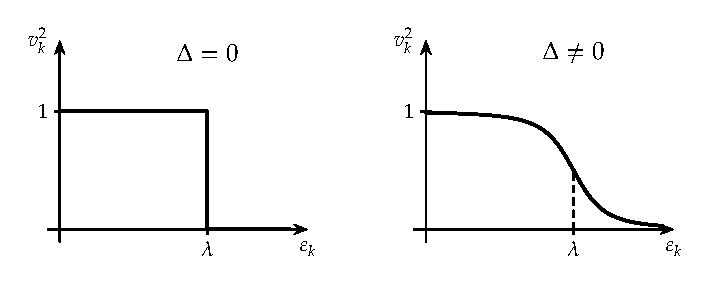
\includegraphics[width=0.7\linewidth]{pictures/6_5}
\par\end{centering}
\centering{}\caption{\label{fig:=0065E0=0076F8=004E92=004F5C=007528=00548C=006709=0076F8=004E92=004F5C=007528=0065F6=007684=005360=00636E=006982=007387}无相互作用$\Delta=0$和有相互作用$\Delta\protect\neq0$时的占据概率}
\end{figure}

\[
\Delta=\frac{G}{2}\sum_{k>0}\frac{\Delta}{\sqrt{(\varepsilon_{k}-\lambda)^{2}+\Delta^{2}}}
\]

在单$j$壳的特殊情况下，所有的$\varepsilon_{k}$都是相等的。从\ref{eq:formal solution of BCS equation G}\ref{eq:tilde epsilon G}和\ref{eq:formal solution of BCS eq}甚至是保留$Gv^{2}_{k}$的情况我们都可以看出，所有的$v^{2}_{k}$都是相等的。从粒子数守恒的条件\ref{eq:particle number expectation}，我们可以得到：
\begin{equation}
v_{k}=\sqrt{\frac{N}{2\Omega}},\quad u_{k}=\sqrt{1-\frac{N}{2\Omega}}\label{eq:v and u G}
\end{equation}

相应的能量（$\varepsilon_{k}=0$）为：
\[
E^{(N)}_{\text{BCS}}=-\frac{1}{2}GN\Omega\left(1-\frac{N}{2\Omega}+\frac{N}{2\Omega^{2}}\right)
\]

这一表达式和精确的结果\ref{eq:E to N}相比，对于大$N$的情况，至少对$1/\Omega$阶的情况是正确的。因此，我们可以说BCS拟设是一个好的近似，非常适合用来处理原子核对关联。

粒子数的不确定度\ref{eq:uncertainty of particle number}也可以从\ref{eq:v and u G}中得到：
\[
\frac{\Delta N}{N}=\frac{1}{\sqrt{N}}\sqrt{2-\frac{N}{\Omega}}
\]

这一模型的能隙可以由\ref{eq:Delta G}和\ref{eq:v and u G}给出：
\[
\Delta=G\sqrt{\frac{N}{2}\left(\Omega-\frac{N}{2}\right)}
\]

因此能隙关于壳中的粒子数是抛物线型的依赖，当壳是空的或者满的的时候，能隙均为零。对于$N=\Omega$，也就是半满壳，我们发现：
\[
2\Delta=G\Omega
\]

我们接下来会看到\ref{subsec:Bogoliubov=0051C6=007C92=005B50=002014=002014=006FC0=0053D1=006001=00548C=00963B=00585E}，$2\Delta$不是偶然的等于第一激发态的能量\ref{eq:energy gap}，随之$\Delta$被称作能隙的原因也会更清晰。

\subsection{Bogoliubov准粒子——激发态和阻塞\label{subsec:Bogoliubov=0051C6=007C92=005B50=002014=002014=006FC0=0053D1=006001=00548C=00963B=00585E}}

把基态写成\ref{eq:BCS wave function}或者\ref{eq:BCS wave function sum form}的形式，除了有和辛弱数模型的精确基态（对的凝聚态）十分相似，因此包含了对关联这一好处之外，还有一个好处就是$|\text{BCS}\rangle$态也可以写成一种新型费米子即Bogoliubov准粒子的直积态。多体物理中的准粒子的概念将会在\ref{chap:=0063A8=005E7F=007684=005355=007C92=005B50=006A21=00578B=00FF08HFB=007406=008BBA=00FF09}中讨论。事实上，可以容易的验证：
\[
|\text{BCS}\rangle\propto\prod_{k}\alpha_{k}|\rangle
\]

这里：
\begin{align}
\alpha^{\dagger}_{k} & =u_{k}a^{\dagger}_{k}-v_{k}a_{\bar{k}}\nonumber \\
\alpha^{\dagger}_{\bar{k}} & =u_{k}a^{\dagger}_{\bar{k}}+v_{k}a_{k}\label{eq:quasi particle operator}
\end{align}

它们满足费米子对易关系：
\[
\{\alpha_{k},\alpha_{k^{\prime}}\}=0;\quad\{\alpha_{k},\alpha^{\dagger}_{k^{\prime}}\}=\delta_{kk^{\prime}}
\]

这里我们通常使用\ref{eq:conj state}和通常的相位约定：
\[
u_{\bar{k}}=u_{k}>0;\quad v_{\bar{k}}=-v_{k}<0;\quad k>0
\]

上式\ref{eq:quasi particle operator}中的拟设和Lipkin模型中的HF-准粒子拟设\ref{eq:Lipkin model operator}非常接近。因此我们可以用相同的技巧来得到解。在Lipkin模型中，我们可以得到实系数（$\varphi=0$）给出了最低能量。在这里，只要$\bar{v}_{k\bar{k}k^{\prime}\bar{k}^{\prime}}<0$，就会出现同样的情况，而这时非常合理的，因此我们只需要使用实系数$u_{k}$和$v_{k}$。

从\ref{eq:quasi particle operator}和\ref{eq:formal solution of BCS eq}我们可以看到，准粒子既有裸粒子的性质，也有裸空穴的性质：在费米面之上（$v^{2}_{k}$很小），它几乎是粒子，而在费米面之下（$u^{2}_{k}$很小），它有几乎是空穴。

从方程\ref{eq:quasi particle operator}可以看出，通过利用线性Bogoliubov变换这个有用的技巧，我们把基态从成对的相互作用粒子表示成了无相互作用准粒子气体。这在很多情况下是非常有用的。而我们必须为之付出的代价则是粒子数不再守恒了——因为我们混合了产生算符和湮灭算符。如果我们假设不仅仅是基态可以由准粒子直积态表示，激发态也可以，那么无相互作用准粒子气体的Hamilton
量$H_{\text{qp}}$则可以表示为：
\[
H_{\text{qp}}=\langle\text{BCS}|H^{\prime}|\text{BCS}\rangle+\sum_{k}E_{k}\alpha^{\dagger}_{k}\alpha_{k}
\]

这里常数$\langle H^{\prime}\rangle$充分考虑了以下事实：
\[
\alpha_{k}|\text{BCS}\rangle=0,\quad\text{对所有的}k
\]

因此，$H_{\text{qp}}$有着正确的基态能量期待值。准粒子能量$E_{k}$是真实粒子相关概念的推广（具体的计算参考\ref{chap:=0063A8=005E7F=007684=005355=007C92=005B50=006A21=00578B=00FF08HFB=007406=008BBA=00FF09}）。
\begin{align*}
E_{k} & =\langle\text{BCS}|\alpha_{k}H^{\prime}\alpha^{\prime}_{k}|\text{BCS}\rangle-\langle\text{BCS}|H^{\prime}|\text{BCS}\rangle\\
 & =\sqrt{\tilde{\varepsilon}^{2}_{k}+\Delta^{2}_{k}}
\end{align*}
 单准粒子态为：
\begin{align*}
\alpha^{\dagger}_{k_{1}}|\text{BCS}\rangle & =a^{\dagger}_{k_{1}}\prod_{k\neq k_{1}}(u_{k}+v_{k}a^{\dagger}_{k}a^{\dagger}_{\bar{k}})|\rangle\\
\alpha^{\dagger}_{\bar{k}_{1}}|\text{BCS}\rangle & =a^{\dagger}_{\bar{k}_{1}}\prod_{k\neq k_{1}}(u_{k}+v_{k}a^{\dagger}_{k}a^{\dagger}_{\bar{k}})|\rangle
\end{align*}

这些态显然有能量为$\langle H^{\prime}\rangle+E_{k}$。它们是具有奇数粒子数的一系列态的叠加，描述了奇核。根据量子数$k_{1}$，这一态既可能是基态，也可能是激发态\footnote{什么意思？可能是奇核的基态或者偶核的激发态？}。

两粒子准粒子态：
\begin{align*}
\alpha^{\dagger}_{k_{1}}\alpha^{\dagger}_{k_{2}}|\text{BCS}\rangle & =a^{\dagger}_{k_{1}}a^{\dagger}_{k_{2}}\prod_{k\neq k_{1},k_{2}}(u_{k}+v_{k}a^{\dagger}_{k}a^{\dagger}_{\bar{k}})|\rangle,\quad k_{2}\neq\bar{k}_{1}\\
\alpha^{\dagger}_{k_{1}}\alpha^{\dagger}_{\bar{k}_{1}}|\text{BCS}\rangle & =(-v_{k_{1}}+u_{k_{1}}a^{\dagger}_{k_{1}}a^{\dagger}_{\bar{k}_{1}})\prod_{k\neq k_{1}}(u_{k}+v_{k}a^{\dagger}_{k}a^{\dagger}_{\bar{k}})|\rangle,\quad k_{2}=\bar{k}_{1}
\end{align*}

它们具有能量$\langle H^{\prime}\rangle+E_{k_{1}}+E_{k_{2}}$。它们描述了偶核的激发态。在这种情况下，有一个对被拆开了，激发能为：
\[
E_{k_{1}}+E_{k_{2}}\ge2\Delta
\]

偶核的第一激发态的能量因此一定比基态能量高出$2\Delta$以上。

在只有一个$j$-壳的情况下，激发能为：
\[
E_{k}+E_{k^{\prime}}=2\sqrt{\tilde{\varepsilon}^{2}+\Delta^{2}}
\]

考虑纯对力的情况，再令$\varepsilon_{k}=0$
\begin{comment}
令$\varepsilon_{k}=0$相当于辛弱数模型。
\end{comment}
，得到：

\[
\tilde{\varepsilon}=G\frac{\Omega-N}{2}
\]

\begin{booknote*}
利用$v^{2}_{k}$的表达式\ref{eq:formal solution of BCS equation G}，得到：
\[
\lambda^{2}=\frac{(2v^{2}_{k}-1)^{2}\Delta^{2}}{1-(2v^{2}_{k}-1)^{2}}
\]

再代入上一节得到的$v^{2}_{k}$和$\Delta$的表达式，得到：
\[
\lambda^{2}=\frac{G^{2}}{4}(N-\Omega)^{2}
\]

由于此时$\tilde{\varepsilon}=-\lambda$，而$\tilde{\varepsilon}$一定为正，所以得到$\tilde{\varepsilon}=G\frac{\Omega-N}{2}$。
\end{booknote*}
从而得出：

\[
E_{k}+E_{k^{\prime}}=G\cdot\Omega
\]

和辛弱数模型得到的结果\ref{eq:energy gap}相符
\begin{comment}
但这是省略了$Gv^{2}_{k}$和$Gv^{4}_{k}$得到的结果。
\end{comment}
。此外由准粒子能$\tilde{\varepsilon}$的表达式我们还可以发现，只有半满壳的时候，激发能才为$2\Delta$。

在基态奇粒子数的系统里，激发态为$\alpha^{\dagger}_{k}|\text{BCS}\rangle$，基态为$\alpha_{k_{0}}|\text{BCS}\rangle$，如果$\tilde{\varepsilon}_{k_{0}}\simeq0$，则激发能为：
\[
E_{k}-E_{k_{0}}=\sqrt{\tilde{\varepsilon}^{2}_{k}+\Delta^{2}}-\Delta
\]

如果$\tilde{\varepsilon}_{k}\ll\Delta$，上式基本为零，我们因此发现在这些奇粒子数系统中能级密度非常大。

我们也可以用如下的方式解释奇偶质量效应：对于任意的$N$，基态能量$E^{\text{GS}}_{N}$可以如下给出：
\[
E^{\text{GS}}_{N+2}=E^{\text{GS}}_{N}+2\lambda;\quad E^{\text{GS}}_{N+1}=E^{\text{GS}}_{N}+\lambda+E_{k_{0}}
\]

因此奇偶质量差为：
\[
\frac{1}{2}[E^{\text{GS}}_{N+2}-E^{\text{GS}}_{N+1}-(E^{\text{GS}}_{N+1}-E^{\text{GS}}_{N})]=-E_{k_{0}}\simeq-\Delta
\]

上式经常用来从实验上测得的结合能确定能隙。现在已经发现，平均来讲能隙和核子数的关系为$\Delta=12\cdot A^{-1/2}$\cite{NA62,ZGS67}，如\ref{fig:=008D28=005B50=0080FD=009699=00968F=008D28=005B50=006570=007684=0053D8=005316(=00005BBM-69=00005D)}。

\begin{figure}[H]
\begin{centering}
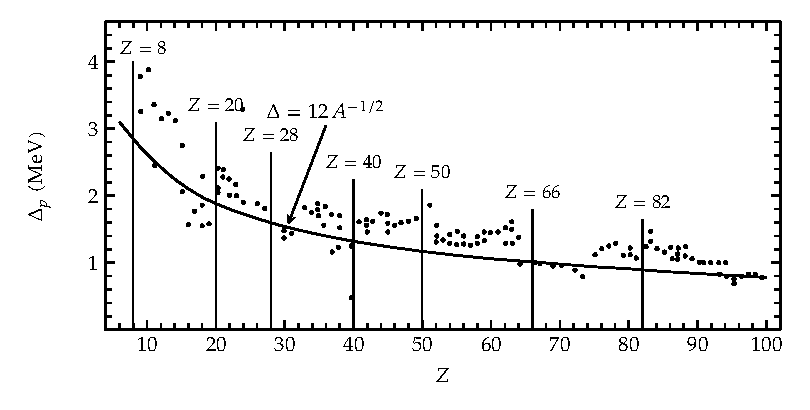
\includegraphics[width=0.6\linewidth]{pictures/6_6}
\par\end{centering}
\centering{}\caption{\label{fig:=008D28=005B50=0080FD=009699=00968F=008D28=005B50=006570=007684=0053D8=005316(=00005BBM-69=00005D)}质子能隙随质子数的变化(\cite{BM69})}
\end{figure}

上述讨论使我们对超流核中许多态的结构获得了定性的理解。然而，在更深入的细致研究中，还有几个重要的要点必须予以考虑：

\textbf{(i) 化学势}（The Chemical Potential）。正如在式\ref{eq:particle number expectation}中所见，化学势$\lambda$的确定是为了使
BCS 基态中的平均粒子数具有正确的数值。利用同一个$\lambda$，对于单准粒子态$|k\rangle=\alpha^{\dagger}_{k}|\text{BCS}\rangle$，我们发现
\begin{equation}
\langle k|\hat{N}|k\rangle=N+u^{2}_{k}-v^{2}_{k}\label{eq:average_particle_number_quasi}
\end{equation}
只有对于远离 Fermi 面的能级$k$，上式才等于$N\pm1$。对于 Fermi 面附近的能级，平均粒子数是不正确的。由于能量对平均粒子数具有强烈的依赖性，因此应当针对奇核中的不同能级以及偶核中的激发能级重新调整化学势$\lambda$。只要我们尚未进行这种重新调整，就应当在计算激发能时使用算符$H^{\prime}=H-\lambda\hat{N}$而不是$H$（正如我们目前所做的那样）。例如，如果我们对式\ref{eq:average_particle_number_quasi}中态$|k\rangle$不正确的粒子数进行修正，就可以看出这一点：
\begin{align*}
E^{k}_{N+1} & =\langle k|H|k\rangle+\frac{\mathrm{d}E}{\mathrm{d}N}(N+1-\langle k|\hat{N}|k\rangle)\\
 & =\langle k|H-\lambda\hat{N}|k\rangle+\lambda(N+1)\\
 & =E^{\text{GS}}_{N}+\lambda+E_{k}
\end{align*}

\textbf{(ii) 阻塞效应}（The Blocking Effect）。BCS 基态的占据概率$v^{2}_{k}${[}式\ref{eq:formal solution of BCS eq}{]}
是由变分原理决定的。奇核系统的基态由如下波函数描述：
\begin{equation}
\alpha^{\dagger}_{k_{1}}|\text{BCS}\rangle=a^{\dagger}_{k_{1}}\prod_{k\neq k_{1}}(u_{k}+v_{k}a^{\dagger}_{k}a^{\dagger}_{\bar{k}})|-\rangle\label{eq:blocked_wavefunction}
\end{equation}
未配对的粒子处在能级$k_{1}$上并将该能级“阻塞”。Pauli 原理阻止了该能级参与由对关联引起的核子散射过程。能级$k_{1}$始终保持被占据，而能级$\bar{k}_{1}$则始终保持为空。只有对于$k\neq k_{1}$，我们才有$v^{2}_{k}=v^{2}_{\bar{k}}$（\ref{fig:=0072B6=006001k1=007684=00963B=00585E}）。将受阻塞的波函数\ref{eq:blocked_wavefunction}作为试探波函数用于变分原理，我们得到与之前相同的关于$v^{2}_{k}$的方程。唯一的区别在于，在能隙的计算中有一个能级被“阻塞”：
\begin{equation}
\Delta=G\sum_{k\neq k_{1}}u_{k}v_{k}\label{eq:blocked_gap}
\end{equation}
能级$k_{1}$必须从求和中排除，因为它无法对配对能量做出贡献。化学势由下式决定：
\begin{equation}
N=1+2\sum_{k\neq k_{1}}v^{2}_{k}\label{eq:blocked_particle_number}
\end{equation}
对于存在更多阻塞能级的情况（例如双准粒子态），完全类似的方程同样成立。

\begin{figure}[H]
\begin{centering}
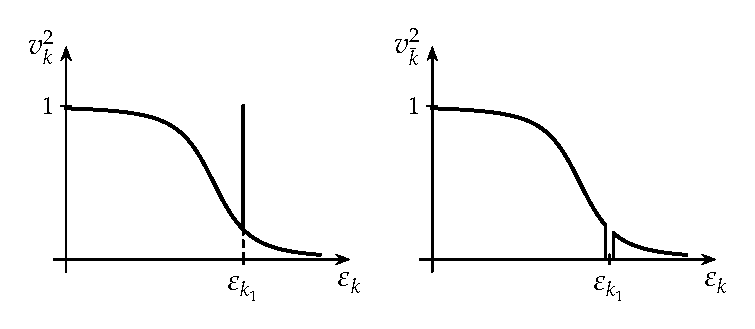
\includegraphics[width=0.85\linewidth]{pictures/6_7}
\par\end{centering}
\centering{}\caption{\label{fig:=0072B6=006001k1=007684=00963B=00585E}状态$k_{1}$的阻塞}
\end{figure}

$\Delta$以及$u_{k}$与$v_{k}$的这种改变称为阻塞效应。这些阻塞关联是$\Omega^{-1}$量级的，通常可以忽略。然而，正如
Soloviev \cite{So61,Wa62b} 以及 Nilsson 和 Prior \cite{NP61} 所指出的，在某些情况下这一修正可能相当大。这在形变核中尤为突出，因为在形变核的能谱中尽管可能有
20 个能级，但对式\ref{eq:gap equation}的求和有显著贡献的仅有 4 或 5 个能级。显然，在这样的情形下阻塞其中一两个能级会产生巨大的影响，以至于人们不能简单地将激发能等同于准粒子能量，而必须计算激发态的总能量并减去真空态能量。对于双准粒子态，修正后的能量（$\simeq1.4\,\text{MeV}$）总是小于准粒子能量（$\simeq1.7\,\text{MeV}$），但远大于自由粒子能量（$\simeq0.15\,\text{MeV}$）。在这种修正理论中产生的一个问题是，$v_{k}$在基态和激发态中可能存在显著差异，导致这些态不再自动正交，尽管有时不同的量子数（如自旋或宇称）能够保证正交性。特别是，在这些情况下自旋为$0^{+}$的双准粒子态与基态并不正交。

\subsection{能隙方程的讨论\label{subsec:=0080FD=009699=0065B9=007A0B=007684=008BA8=008BBA}}

在所有实际应用中，BCS 方程都必须借助计算机进行数值求解，于是就产生了一个问题：在计算中应当包含多少个能级？也就是说，我们必须探究哪些状态对能隙方程\ref{eq:gap equation}中出现的求和贡献最大。为此，让我们首先考虑靠近
Fermi 能级的某个状态的能隙$\Delta_{k}$。在这种情况下，求和的主要贡献来自 Fermi 能级附近的状态。其原因在于：(i)
在此情形下，表达式$\Delta_{k^{\prime}}/(\tilde{\varepsilon}^{2}_{k^{\prime}}+\Delta^{2}_{k^{\prime}})^{1/2}\simeq1$（因为$\tilde{\varepsilon}_{k^{\prime}}\simeq0$）；(ii)
当$k^{\prime}\simeq k$时（波函数具有强重叠），矩阵元$\bar{v}_{k\bar{k}k^{\prime}\bar{k}^{\prime}}$比其他矩阵元更大。

反之，若$k$远离 Fermi 面，则式\ref{eq:gap equation}求和中的所有项都很小。对于$k^{\prime}\simeq k$，波函数的重叠虽然仍然很大，但由于$\tilde{\varepsilon}^{2}_{k}\gg\Delta^{2}_{k}$，因子$\Delta_{k^{\prime}}/(\tilde{\varepsilon}^{2}_{k^{\prime}}+\Delta^{2}_{k^{\prime}})^{1/2}$此时变得很小。而对于
Fermi 面上的状态$k^{\prime}$，情况恰好相反，因为那里的矩阵元非常小（$k$与$k^{\prime}$通常属于不同的主量子数）。

因此，配对力的效应局限于 Fermi 面的邻域，也就是说，仅在这一邻域内$\Delta_{k}$才显著不为零。现在我们便能理解，为什么在
Fermi 面邻域取常数配对力而在其余区域矩阵元取为零是一个合理的近似。另一方面，如果我们在整个组态空间中都取常数矩阵元，则能隙将会发散。

对于球形或仅弱形变的原子核，单粒子能级呈现出显著的壳层结构。能隙方程求和中的主要贡献来自于同一壳层内的跃迁。因此，我们或多或少可以分别独立处理各个壳层。由上述讨论，我们预期对于内壳层有$\Delta_{k}\simeq0$。因此，配对力仅在部分填充的壳层中有效，该壳层通常称为$\Lambda$壳层（$\Lambda$-shell）。这便回到了辛弱数模型。对于强形变核，壳层结构已被完全抹平，尽管如此，求和依然仅仅遍及
Fermi 面邻近的一组能级，这组能级同样称为$\Lambda$壳层。

配对效应局限于 Fermi 能级附近，这也是中子与质子可以分别独立处理的原因（至少对于重核而言）。对于$A\sim150$的原子核，过剩中子数为$(N-Z)\geqslant20$。因此，靠近
Fermi 能级的中子与质子能级之间的重叠，与纯质子或纯中子能级之间的重叠相比非常小。因此，忽略中子-质子配对，总波函数可以表示为质子部分与中子部分的直积：
\begin{equation}
|\text{BCS}\rangle=\prod_{k_{1}>0}\left(u^{(p)}_{k_{1}}+v^{(p)}_{k_{1}}a^{(p)\dagger}_{k_{1}}a^{(p)\dagger}_{\bar{k}_{1}}\right)\prod_{k_{2}>0}\left(u^{(n)}_{k_{2}}+v^{(n)}_{k_{2}}a^{(n)\dagger}_{k_{2}}a^{(n)\dagger}_{\bar{k}_{2}}\right)|-\rangle\label{eq:bcs_proton_neutron}
\end{equation}

尽管引入了这些简化假设，BCS 方程通常仍只能通过数值计算求解。为了定性地研究核子对之间相互作用的影响，我们将自身限制于$\Lambda$壳层内的纯配对力\ref{eq:pure pair force energy expectation}。在接下来的讨论中，我们因而忽略其他壳层。此时能隙方程具有如下形式：
\begin{equation}
\Delta=\frac{1}{2}G\sum^{\Lambda}_{k>0}\frac{\Delta}{\sqrt{\tilde{\varepsilon}^{2}_{k}+\Delta^{2}}}\label{eq:gap_equation_lambda_shell}
\end{equation}
其中求和仅遍历$\Lambda$壳层。方程\ref{eq:gap_equation_lambda_shell}总是存在平凡解$\Delta=0$，即$u_{k}\cdot v_{k}=0$；在不存在配对力或配对力足够弱时，这是唯一的解。然而，当满足条件
\begin{equation}
\frac{1}{2}G\sum^{\Lambda}_{k>0}\frac{1}{|\tilde{\varepsilon}_{k}|}>1\label{eq:nontrivial_gap_condition}
\end{equation}
时，存在第二个非平庸解$\Delta>0$。只要配对力足够强，或者$\Lambda$壳层足够大，这种情况总会发生。然而，这一突变的相变是粒子数不守恒（粒子数破缺）的结果，在更扩展的理论
\cite{MPR65} 中它在某种程度上会被抹平平滑化。对于无限大系统，粒子数破缺是可以忽略的，此时相变总是尖锐突变的。

另一方面，式\ref{eq:gap_equation_lambda_shell}也可用于确定配对力的强度$G$，因为正如我们之前所述，$\Delta$可以从奇偶效应经验地确定。然而，它仍然依赖于“截断”（cutoff）$\Lambda$。

\subsection{能隙方程的示意解\label{subsec:=0080FD=009699=0065B9=007A0B=007684=00793A=00610F=0089E3}}

获得能隙方程的解析解是非常富有启发性的 \cite{Be59}。这只能在一个非常简化的示意模型中实现。我们设想一个具有良好形变的原子核，其能级密度近似均匀，且平均能级间距$\Delta\varepsilon$远小于$\Delta$（对于稀土区的形变核，$\Delta\simeq1\,\text{MeV}$，而$\Delta\varepsilon\simeq0.1\text{--}0.2\,\text{MeV}$）。于是我们可以近似地将式\ref{eq:gap_equation_lambda_shell}中的求和替换为在$\Lambda$壳层上的积分：$\varepsilon^{\prime}<\varepsilon<\varepsilon^{\prime\prime}$；令$a=\varepsilon^{\prime}-\lambda$，$b=\varepsilon^{\prime\prime}-\lambda$，有
\begin{equation}
1=\frac{1}{2}G\int^{b}_{a}\frac{1}{\sqrt{\varepsilon^{2}+\Delta^{2}}}\rho(\varepsilon)\,\mathrm{d}\varepsilon\label{eq:schematic_gap_integral}
\end{equation}
其中$\rho(\varepsilon)$为能级密度。我们进一步假设$\rho(\varepsilon)$在$\Lambda$壳层内近似为常数（$\rho\simeq\bar{\rho}$）。引入无量纲量
\begin{equation}
\eta=\frac{1}{\bar{\rho}G}\label{eq:eta_definition}
\end{equation}
积分后可得
\begin{equation}
2\eta=\operatorname{arsinh}\frac{b}{\Delta}-\operatorname{arsinh}\frac{a}{\Delta}\label{eq:arsinh_relation}
\end{equation}
解出$\Delta$可得
\begin{equation}
\Delta=\frac{1}{\sinh2\eta}\sqrt{b^{2}+a^{2}-2ab\cosh2\eta}\label{eq:delta_schematic_solution}
\end{equation}
BCS 模型中的平均粒子数由式\ref{eq:particle number expectation}给出，并由此确定化学势$\lambda$。$\Lambda$壳层内的粒子数由下式给出（我们再次将式\ref{eq:particle number expectation}中的求和替换为积分）：
\begin{equation}
N=2\int^{b}_{a}\frac{1}{2}\left(1-\frac{\varepsilon}{\sqrt{\varepsilon^{2}+\Delta^{2}}}\right)\bar{\rho}\,\mathrm{d}\varepsilon\label{eq:particle_number_schematic}
\end{equation}
$\Lambda$壳层内的能级数由下式给出：
\begin{equation}
\Omega=\bar{\rho}(b-a)\label{eq:omega_levels}
\end{equation}
引入占据因子
\begin{equation}
\chi_{N}=1-\frac{N}{\Omega}\label{eq:chi_n_definition}
\end{equation}
利用式\ref{eq:delta_schematic_solution}，经过冗长但直接的计算，可得
\begin{equation}
\lambda=\frac{\varepsilon^{\prime}+\varepsilon^{\prime\prime}}{2}-\frac{\varepsilon^{\prime\prime}-\varepsilon^{\prime}}{2}\chi_{N}\operatorname{ctgh}\eta\label{eq:lambda_schematic}
\end{equation}
将式\ref{eq:lambda_schematic}代入式\ref{eq:delta_schematic_solution}，得到：
\begin{equation}
\Delta=\frac{\varepsilon^{\prime\prime}-\varepsilon^{\prime}}{2\sinh\eta}\sqrt{1-\chi^{2}_{N}}\label{eq:delta_chi_n}
\end{equation}
在弱耦合极限下，即对于$G\cdot\bar{\rho}\ll1$，我们发现：
\begin{equation}
\Delta\propto\mathrm{e}^{-(1/\bar{\rho}G)}\label{eq:delta_exponential_weak}
\end{equation}
因此，从式\ref{eq:delta_exponential_weak}可以得到一个重要结论：能隙不能按相互作用强度的幂级数展开。

式\ref{eq:delta_chi_n}是在$\Delta$不小于能级间距的条件下导出的，即
\begin{equation}
\Delta\cdot\bar{\rho}>1\label{eq:delta_rho_condition}
\end{equation}
或者
\begin{equation}
\frac{1}{2\sinh\eta}\sqrt{N(2\Omega-N)}>1\label{eq:delta_rho_condition_explicit}
\end{equation}
对于$\eta\ll1$（强配对关联），该不等式总是满足的。对于$\eta\gg1$，式\ref{eq:delta_rho_condition_explicit}仅在$N(2\Omega-N)$的值足够大时才成立。

BCS 理论中的基态能量由式\ref{eq:pure pair force energy expectation}给出。它对$H^{\prime}$的基态期望值的贡献为
\begin{equation}
\langle\text{BCS}|H^{\prime}|\text{BCS}\rangle=2\int^{b}_{a}\frac{1}{2}\left(1-\frac{\varepsilon}{\sqrt{\varepsilon^{2}+\Delta^{2}}}\right)\varepsilon\bar{\rho}\,\mathrm{d}\varepsilon-\frac{\Delta^{2}}{G}\label{eq:h_prime_expectation}
\end{equation}
由于$H^{\prime}$与$H$相差$\lambda\cdot N$，利用式\ref{eq:lambda_schematic}并完成式\ref{eq:h_prime_expectation}中的积分，我们得到基态能量：
\begin{equation}
E_{\text{BCS}}=\langle\text{BCS}|H|\text{BCS}\rangle=\frac{1}{2}(\varepsilon^{\prime\prime}+\varepsilon^{\prime})N-\frac{1}{4}\Omega(\varepsilon^{\prime\prime}-\varepsilon^{\prime})(1-\chi^{2}_{N})\operatorname{ctgh}\eta\label{eq:e_bcs_energy}
\end{equation}
我们关注的是基态能量中单纯来自配对力的那一部分。为此，我们首先计算$G=0$时的能量，这对应于极限$\eta\to\infty$：
\begin{equation}
E^{0}=\frac{1}{2}(\varepsilon^{\prime}+\varepsilon^{\prime\prime})\cdot N-\frac{1}{4}\Omega(\varepsilon^{\prime\prime}-\varepsilon^{\prime})(1-\chi^{2}_{N})\label{eq:e_zero_energy}
\end{equation}
因此，配对力对基态能量的贡献$E^{P}$由下式给出：
\begin{equation}
E^{P}=E_{\text{BCS}}-E^{0}\label{eq:e_p_definition}
\end{equation}
在半满壳层（即$N=\Omega$）的情形下，利用式\ref{eq:e_bcs_energy}、式\ref{eq:e_zero_energy}、式\ref{eq:omega_levels}和式\ref{eq:delta_chi_n}，可得
\begin{equation}
E^{P}=-\frac{1}{4}\Omega(\varepsilon^{\prime\prime}-\varepsilon^{\prime})(1-\chi^{2}_{N})(\operatorname{ctgh}\eta-1)=-\frac{1}{2}\Delta^{2}\bar{\rho}(1-\mathrm{e}^{-2\eta})\label{eq:e_p_half_filled}
\end{equation}
这就是中子或质子的配对能（pairing energy）。对于重核，可以从奇偶效应估计$G$和$\Delta$。Nilsson
和 Prior \cite{NP61} 发现，对于质子$G_{p}\simeq17/A\,\text{MeV}$，对于中子$G_{n}\simeq25/A\,\text{MeV}$。能隙$\Delta$约为$1\,\text{MeV}$。假设特征能级密度为$1/\bar{\rho}\simeq0.5\,\text{MeV}$，可得$\eta\simeq A/100$。在此情形下，我们可以忽略式\ref{eq:e_p_half_filled}中的$\mathrm{e}^{-2\eta}$项，从而得到总配对能（质子和中子的配对能大致相同）：
\begin{equation}
E^{P}_{\text{total}}=E^{P}_{(p)}+E^{P}_{(n)}\simeq-\bar{\rho}\Delta^{2}\simeq-2\,[\text{MeV}]\label{eq:e_total_pairing}
\end{equation}
因此，与总结合能相比，总配对能极其微小。这是各类关联能的普遍特征，然而，这绝不意味着它们在解释许多物理问题时不能发挥决定性的作用。

正如我们所见，BCS 波函数所代表的态并不是粒子数算符的本征态。整个理论仅在$|\text{BCS}\rangle$很好地定域于实际粒子数附近时才有效。为了获得一个估计，我们计算粒子数的均方偏差\ref{eq:uncertainty of particle number}：
\begin{equation}
(\Delta N)^{2}=\sum_{k>0}\frac{\Delta^{2}_{k}}{\tilde{\varepsilon}^{2}_{k}+\Delta^{2}_{k}}\label{eq:delta_n_squared_definition}
\end{equation}
在示意模型中，由此可得
\begin{equation}
(\Delta N)^{2}=\bar{\rho}\Delta\left(\arctan\frac{b}{\Delta}-\arctan\frac{a}{\Delta}\right)\label{eq:delta_n_squared_schematic}
\end{equation}
在弱配对关联或低能级密度的极限下，我们得到
\begin{equation}
(\Delta N)^{2}=\bar{\rho}\cdot\Delta\cdot\pi\label{eq:delta_n_weak_pairing}
\end{equation}
这一近似对于强形变核大体上是满足的。取$\bar{\rho}$和$G$的典型特征值，我们得到$\eta\simeq4,\dots,5$，平均偏差为$\Delta N\simeq\sqrt{6}$。

在强配对的另一极限下（$\eta\ll1$），我们仅保留式\ref{eq:delta_n_squared_schematic}关于$\eta$的领头项：
\begin{equation}
(\Delta N)^{2}=\Omega(1-\chi^{2}_{N})=2N\left(1-\frac{N}{2\Omega}\right)\label{eq:delta_n_strong_pairing}
\end{equation}
因此，对于半满壳层（$N=\Omega$），可得$\Delta N=\sqrt{N}$；而对于仅有一对核子（$N=2$），我们得到$\Delta N\simeq2$。$\eta\ll1$的半满壳层的一个典型例子是$^{202}\text{Pb}$。其
BCS 波函数包含大量的$^{204}\text{Pb}$和$^{200}\text{Pb}$，以及$^{206}\text{Pb}$和$^{198}\text{Pb}$。然而我们必须记住，对于所有这些核，Fermi
面$\lambda$和能隙$\Delta$几乎完全相同，因此粒子数的不确定性并不像表面上看起来那么严重。

正如我们所看到的，非常简单的 BCS 模型使我们能够解释核子短程关联所引起的原子核的许多特征。我们仅分别独立处理了中子和质子的配对，忽略了中子-质子相互作用。对于重核，这是合理的，因为质子和中子波函数通常属于不同的主量子数，配对矩阵元很小。然而对于轻核（$s\text{--}d$壳层！），这不再成立，我们还必须计入中子-质子配对。在非常简要地提及其中某些计算之前，我们希望从更一般的
Hartree-Fock-Bogoliubov 理论重新审视 Hartree-Fock 理论、形变以及配对，正如我们将看到的，该理论涵盖了我们迄今所讨论的所有模型。
